\documentclass{article}

\usepackage{graphicx}
\usepackage{subfigure}
\usepackage[hypcap]{caption}
\usepackage{listings}
\usepackage{float}
\floatstyle{plaintop}
\restylefloat{table}

\title{Experimental Design and Data Analysis: Assignment 2}
\author{Andrew Bedard \& Simone van Gompel(2567525) \\ Group 19}

\begin{document}

  \maketitle

  \section{Exercise 1}
  	Look at Fig:\ref{fig:Pairs} for the pairwise graph....

    \begin{figure}
      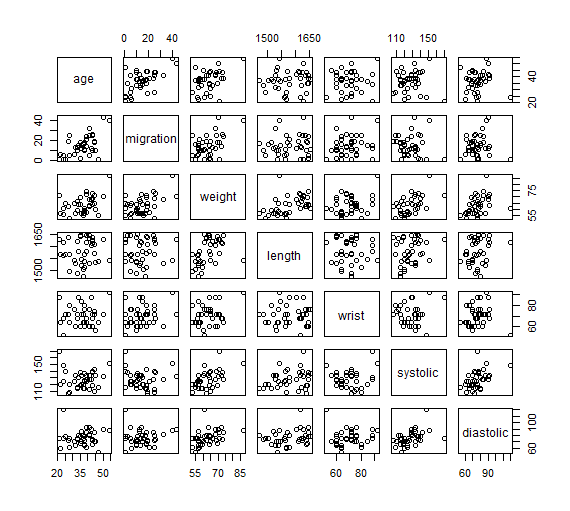
\includegraphics[scale=0.6]{../results/Pairs.png}
      \caption{Pairwise scatterplots of the dataset peruvians}
      \label{fig:Pairs}
    \end{figure}
\end{document}